%\santi{Para mi esto debería estar antes. Principalmente porque ya aparecio una red bayesiana en la demo anterior. Capaz podes ponerlo pegado a la seccion 3.1, que es también medio introductoria. Sino también puede ir antes}

\begin{comment}
    Una Red Bayesiana para features \(X\) es una tupla \(\aBayesianNetwork = (X, E, \Pr)\), donde \((X, E)\) es un DAG que tiene los features \(X\) como nodos, $E$ sus aristas y \(\Pr\) es una función que codifica, para cada feature \(X\), su distribución de probabilidad condicional \(\Pr(X | \parents(X))\). La semántica topológica especifica que cada variable es condicionalmente independiente de sus no-descendientes, dado sus padres (y es por esto que la información de \(\Pr\) es suficiente para reconstruir la distribución conjunta de \(X\)).

\echu{¿Tiene sentido poner esta definición acá si después vamos a definirlo de vuelta en la siguiente sección? Podemos poner sólo la de la naive bayes sin tener en cuenta la de la red bayesiana. }
\sergio{Creo que es mejor evitar repetición directa, y además es mejor si se introducen los nuevos conceptos de manera más gradual cuando tiene sentido}
\santi{Banco a muerte no repetir, pero soy de la escuela de definir todo al principio. Da igual de todas formas.}

Dada una Red Bayesiana \(\aBayesianNetwork\), sea \(\pi \in perm(X)\) un orden topológico para el DAG de \(\aBayesianNetwork\). Entonces, la probabilidad para alguna entidad \(e\) se calcula como \footnote{A partir de ahora, denotamos por \(X_i\) la variable aleatoria asociada al feature \(x_i\).}

\begin{align}\label{eq:bayesian_probability}
    \Pr[e] = \Pr\left[\bigwedge_{i=1}^n X_i = e(x_i)\right] &= \prod_{i=1}^n \Pr\left[X_{\pi(i)} = e(x_{\pi(i)}) | \bigwedge_{i=1}^{i-1} X_{\pi(i)} = e(x_{\pi(i)})\right]\nonumber \\
    &= \prod_{i=1}^n \Pr\left[X_{\pi(i)} = e(x_{\pi(i)}) | \bigwedge_{x_j \in \parents(x_i)} X_j = e(x_j)\right]
\end{align}

donde en la última desigualdad usamos las restricciones topológicas para condicionar únicamente en los padres de \(x_i\). \cite{Darwiche_2009} Esta fórmula se basa en utilizar el teorema de Bayes para descomponer a la conjunción de valores que representa la entidad $e$ en varias probabilidades condicionales utilizando las distintas dependencias entre las variables que tiene un orden tópologico. 

Este modelo se basa en un grafo acíclico dirigido (DAG) donde la variable objetivo \(Y\) es el único nodo padre y todos los features \(X_i\) son hijos independientes. Dado que cualquier familia razonable de modelos contiene este tipo de funciones, la posibilidad de desarrollar algoritmos eficientes para calcular los Shapley values bajo distribuciones bayesianas parece limitada. Aún así hay familias de modelos para los cuáles se puede computar si tenemos una distribución de Markov \cite{marzouk2024tractabilityshapexplanationsmarkovian}.

%\echu{¿Meto esto que esta en el comment en algún lado o ya lo elimino? No se si suma tanto } Rta Cifu: No suma tanto, afueraa esto

\end{comment}

Como mencionamos en la sección anterior, $ASV$ utiliza el grafo causal asociado al problema para definir una función $w$, que nos va a permitir filtrar permutaciones no deseadas que no respeten la causalidad. Luego, cuando tenemos una permutación $\topo$ que sí nos interesa, vamos a querer realizar la operación $\charactheristicFunction(\pi_{<i})$, la cual consiste en evaluar la esperanza teniendo en cuenta nuestra distribución elegida y un valor fijo para los features en $\pi_{<i}$. Para realizar este cálculo necesitamos entender cómo se calculan probabilidades en una red bayesiana y cuál es su complejidad. 

\subsection{Redes Bayesianas}
Una Red Bayesiana $\aBayesianNetwork$ es un $DAG$, donde cada nodo representa una variable diferente y los arcos representan las dependencias condicionales entre ellas, puesto que para calcular la probabilidad de la cabeza necesitamos la de la cola. Por ejemplo, si tenemos el arco $A \longrightarrow B$, esto representa que la variable $B$ depende\footnote{Aunque no necesariamente significa que $A$ dependa de $B$ causalmente, puesto que podríamos armar una red bayesiana que no se condiga con el DAG causal de las variables. } de $A$, y esto se cuantifica usando la probabilidad condicional $P(B|A)$. Un nodo puede tener múltiples padres, por lo que la distribución de los valores del nodo se definirá en una \emph{Tabla de Probabilidad Condicional} (CPT), que define la probabilidad de que tome algún valor, dado los posibles valores de sus nodos padres. Con esto, podemos definir una Red Bayesiana como:

%\santi{Diría que esto es \textit{Intuitivamente}. Nada impide que armes una red bayesiana con todas las dependencias al revés. El truco es que si respetas la causalidad la red debería quedar con pocos ejes, pero en principio cualquier distribución se puede representar tomando cualquier ordenamiento de las variables aleatorias. La definción correcta correcta es que tenés tablitas, y se definen en función de los padres, y todas las tablas juntas dan una distribución.} Echu : Con dependencias condicionales me refería a que dependen en la probabilidad condicional de sus padres
% \santi{Creo que esto queda mejor en un footnote.}

\begin{definition}
Una Red Bayesiana para variables \(X\) es una tupla \(\aBayesianNetwork = (X, E, \Pr)\), donde \((X, E)\) es un DAG que tiene las variables \(X\) como nodos, $E$ como aristas y \(\Pr\) es una función que codifica, para cada variable \(x \in X\), su distribución de probabilidad condicional \(\Pr(x | \parents(X))\):

\begin{itemize}
    \item Para cada variable $x \in X$, sabemos que $x$ tiene un conjunto finito de estados mutuamente excluyentes. Estos son los posibles valores que puede tomar.
    \item Para cada variable $x \in X$ con padres $B_1, \dots, B_n$, se tiene una tabla de probabilidad condicional (CPT) $Pr(x \mid B_1, \dots, B_n)$. Así es como está definida $Pr$.
\end{itemize}
    
\end{definition}

\begin{figure}[ht]
    \centering
    \includegraphics[scale=0.4]{img/bayesianNetworks/bayesianNetworks.png}
    \caption{Red Bayesiana para determinar la inteligencia de un estudiante. Podemos ver que cada nodo tiene una $CPT$ que se calcula en función de sus padres. Aquí las variables son ternarias o binarias. Fuente: \cite{probabilisticGraphicalModels}}
    \label{fig:bayesian_network_example}
\end{figure}

 
Este tipo de redes nos ayuda a simplificar el cálculo de distribuciones de probabilidad conjunta. Una de sus propiedades más importantes es la \emph{regla de la cadena}, que proporciona una estructura fundamental para entender cómo las probabilidades conjuntas pueden descomponerse en estas redes. Específicamente, establece que si consideramos que $\aBayesianNetwork$ es una red Bayesiana sobre un conjunto de variables \( \{A_1, \dots, A_n\} \), entonces $\aBayesianNetwork$ especifica una única distribución de probabilidad conjunta \( Pr(U) \), donde \( U = \{A_1, \dots, A_n\} \), que puede expresarse como el producto de todas las CPT's especificadas en $\aBayesianNetwork$. Matemáticamente, se representa como:
\begin{align}\label{eq:bayesian_probability}
    Pr(U) = \prod_{i=1}^{n} P(A_i \mid \parents(A_i))    
\end{align}

donde $\parents(A_i)$  denota los padres de \( A_i \) en la red. Esta regla es esencial porque simplifica el cálculo de la distribución de probabilidad conjunta al descomponerla en dependencias locales más simples entre un nodo y sus predecesores directos. Intuitivamente, lo que hace es utilizar las dependencias locales para definir una distribución global, facilitando los procesos de inferencia dentro de estas redes.

%\santi{Acá estamos repitiendo las cosas que ya se dijeron unas páginsa anteriores al hablar por primera vez de redes bayesianas.}

Además, las redes Bayesianas contemplan una variedad de operaciones computacionales cruciales para el razonamiento probabilístico. Una de las operaciones principales es la \textbf{inferencia}, que implica calcular la distribución a priori para alguna variable. Es decir, calcular $Pr(A \mid B_1  \dots B_i)$, siendo $A$ un nodo en la red y $B_i$ otros nodos de la red. Este proceso a menudo se denomina \emph{consulta} a la red. La complejidad de la inferencia depende de la estructura de la red; para redes con forma de polytree (DAG's que su grafo subyacente es un árbol), también conocidas como \emph{simplemente conectadas}, la complejidad es polinomial en el tamaño de las variables de la red \cite{pearl1986bayesianInference}, pero para redes generales la inferencia es $\sharpPhard$. 

%\santi{Hace falta que sean padres? No es en general?} Rta: Es general, pifie

El algoritmo que se utiliza  para realizar la inferencia marginal, que calcula cual es la probabilidad de que una variable tome ciertos valores, es \emph{Variable Elimination} \cite{variableElimination}. Su complejidad depende principalmente del treewidth\footnote{El treewidth (ancho de árbol) de un grafo es una medida de cuán ``cercano´´ está un grafo a ser un polytree. Formalmente, es el tamaño del mayor conjunto de vértices en una descomposición en árbol, menos uno, minimizado sobre todas las posibles descomposiciones.} de la red y puntualmente para redes de un treewidth acotado, su complejidad es polinomial respecto al tamaño de la red. En base a esto es que elegimos trabajar con polytrees. 

%\santi{Hace falta poner la explicación de variable elimination? Al final no lo usamos nunca, no?}

\subsection{Predicción promedio en árboles de decisión}

Los árboles de decisión son ampliamente utilizados en Inteligencia Artificial (IA) debido a su capacidad para realizar predicciones y clasificaciones basadas en features de los datos de entrada. Al descomponer decisiones en una serie de preguntas y respuestas simples, los árboles de decisión permiten a los usuarios entender el razonamiento detrás de las predicciones del modelo, contribuyendo a la transparencia en sistemas complejos \footnote{Aunque no siempre el camino de un árbol es la mejor explicación, ya que puede haber features redundantes en el camino que no sean claves para la predicción realizada. \cite{audemard2021explanatorypowerdecisiontrees}}.
%\santi{Acá agregaría un footnote y una cita comentando que el camino en el árbol no es necesariamente una buena explicación. Hay discusiones sobre esto en papers de abductive explanations para árboles, por ejemplo \url{https://arxiv.org/pdf/2108.05266} (último párrafo pag 2)}

\begin{definition}
Un \textbf{árbol de decisión} es una estructura jerárquica utilizada para representar funciones de decisión sobre un conjunto finito de variables. Formalmente, un árbol de decisión \(T\) sobre un conjunto de variables \(X\) es un árbol enraizado cuyas componentes principales son:

\begin{itemize}
    \item \textbf{Nodos internos}, cada uno asociado a una variable \(x \in X\) y etiquetado con una condición sobre dicha variable. Estos nodos determinan cómo se bifurcan los datos.
    
    \item \textbf{Ramas}, que conectan un nodo padre con sus hijos y representan los posibles valores o resultados de evaluar la condición del nodo padre.
    
    \item \textbf{Hojas}, que son nodos sin hijos y contienen una salida concreta: una clase, un valor numérico, o una distribución de probabilidad, dependiendo del tipo de problema (clasificación, regresión, o probabilístico).
\end{itemize}

Cada instancia \(e \in \entities(X)\) se evalúa recorriendo el árbol desde la raíz hasta una hoja, tomando decisiones en función de las condiciones de los nodos internos. El resultado asociado a la hoja alcanzada es la predicción del modelo para esa instancia.

\end{definition}

Como mencionamos previamente, investigamos si el cálculo del promedio era tratable para árboles de decisión con distribuciones de redes bayesianas, ya que nuestro objetivo era calcular ASV en tiempo polinomial. %\santi{Ídem comentario de más arriba. Hacemos esto porque después lo vamos a necesitar para cacular $v(\pi_{<i})$, no por el Teorema 1, que no dice mucho sobre distribuciones no producto.}%\santi{Reescribiría esta oración.}

%\sidesergio{recordar no poner referencias sueltas, poner Teorema ref. Relacionadamente, por consistencia, capitalizar esas referencias (Teorema, Ecuación, etc.)}

%\santi{Sería un poco más formal en la definición.} 

Para este algoritmo\footnote{Pueden encontrar este algoritmo en \path{\pasantia-BICC\asvFormula\bayesianNetworks\bayesianNetwork.py}} trabajaremos con árboles de decisión binarios y con features binarios, más adelante veremos la extensión a variables no binarias. Cada nodo determinará un valor para un feature $X_i$, donde el hijo izquierdo corresponde al caso $X_i=0$ y el hijo derecho al caso $X_i=1$. Los features son un conjunto $X$, y su distribución de probabilidad será una red bayesiana $\aBayesianNetwork = (V, E, Pr_B)$. Definimos a $ev$ y $pathCondition$ cómo conjuntos de asignaciones $X_i = k$, las cuales definen que el feature $X_i$ toma el valor $k$. Entonces, $Pr_B(pathCondition \mid ev)$ representa la probabilidad de que dada una instancia que tiene los valores de $ev$, la instancia tome los valores de $pathCondition$, dada la red bayesiana $\aBayesianNetwork$. La idea del algoritmo consiste en explorar todas las ramas e ir acumulando las decisiones tomadas en la variable $pathCondition$. Al llegar a la hoja evaluamos la probabilidad de haber llegado a la hoja dada la evidencia y la multiplicamos por el valor que la misma devuelve. 

%\santi{Agregaría un párrafo comentando la idea del algoritmo. Aparte, si asumimos que en ningún camino se repiten features podríamos quitar las líneas 2-4, no? Aunque cuando haya más de un valor para cada feature eso deja de ser cierto. Capaz podemos comentarlo (igual no es muy relevante)}

%\santi{Qué es una evidencia? Estás pisando la $E$ de la definición de la red.}

%\echu{No entendí el comentario de Santi de lo de las líneas 2-4}

%Ya se entendio


\begin{algorithm}
\caption{Predicción promedio para árbol de decisión binario} \label{alg:meanPredBinDT}
\begin{algorithmic}[1]
\Function{Mean}{$node$, $B$, $pathCondition$, $evidence$}
    \If{$evidence$ does not match $pathCondition$}
        \State \Return  $0$
    \EndIf
    
    \If{$node$.isLeaf}
        \State \Return  $Pr_B(pathCondition\ | \ evidence) \cdot node.value$
    \EndIf
    \State $X_i \gets node.feature$
    \State $leftMean \gets$  \Call{Mean}{$node$.left, $B$, $pathCondition \cup \set{X_i=0}, evidence$}
    \State $rigthMean\gets$ \Call{Mean}{$node$.right,$B$,$pathCondition \cup \set{X_i=1}, evidence$} 
    \State \Return  \mbox{$leftMean + rigthMean$}
\EndFunction
\end{algorithmic}
\end{algorithm}

Analicemos la complejidad del Algoritmo \ref{alg:meanPredBinDT}. La condición del primer \texttt{if} puede ser evaluada en tiempo $O(|V|)$. En las hojas solo hacemos un llamado al algoritmo de \textit{variable elimination}, cuya complejidad denotamos como $O(varElim)$. Por otro lado, en los nodos internos solo se hacen los llamados recursivos extendiendo la \textit{pathCondition}, lo cual puede implementarse en $O(1)$. Por lo tanto, si $l$ denota la cantidad de hojas de nuestro árbol de decisión, e $i$ la cantidad de nodos internos, la complejidad de nuestro algoritmo es $O(i|V| + (varElim)l)$. En el caso de los polytrees $varElim$ es polinomial, por lo que nuestro algoritmo realizaría una cantidad de operaciones polinomial en función del tamaño del árbol de decisión, siendo estas ($O(i + l) = O(|V|)$) operaciones polinomiales. %, de costo polinomial $O(varElim) \ y \ O(|V|)$.

%\santi{Lineal?}

%\santi{Definir antes que la red es una tupla (V, E, Pr) y acá directamente poner $O(|V|)$}
%\santi{Ojo que cuando hablaste de VE lo consideraste un algoritmo para evaluar $P(A)$, y ahora querés evaluar $P(A | B)$. Podés directamente introducirlo como algo para calcular $P(A|B)$ y obtenés lo otro como caso particular.}
%\santi{Usaría otra expresión distinta a $VE$}

%\santi{Sobre tu comment en el latex, podés no decir polinomial hasta el final, solo poné las complejidades y aclará que VE es polinomial.}

%¿Polinomial en base a que? ¿Aclaro de vuelta todo lo anterior? Siento que estoy diciendo todo el tiempo lo mismo, necesito sinonimos de polinomial. ¿Lo hago más formal?

\begin{figure}[ht]
    \centering
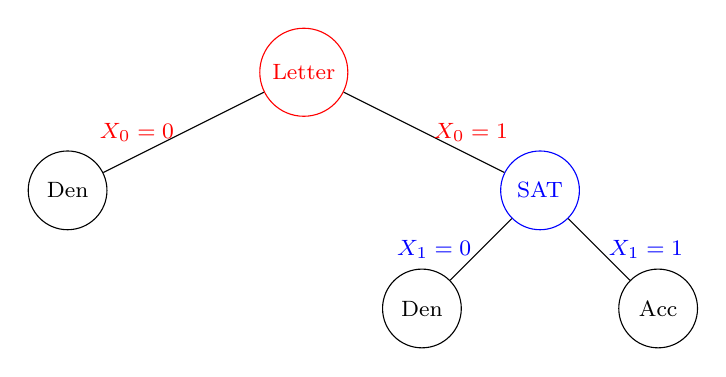
\begin{tikzpicture}[
    level 1/.style={sibling distance=6cm},
    level 2/.style={sibling distance=3cm},
    every node/.style={minimum size=1cm, font=\footnotesize}
]
\node [circle, draw, red] {Letter}
    child {
        node [circle, draw] {Den}
        edge from parent node[left] {\textcolor{red}{$X_0 = 0$}}
    }
    child {
        node [circle, draw, blue] {SAT}
        child {
            node [circle, draw] {Den}
            edge from parent node[left] {\textcolor{blue}{$X_1 = 0$}}
        }
        child {
            node [circle, draw] {Acc}
            edge from parent node[right] {\textcolor{blue}{$X_1 = 1$}}
        }
        edge from parent node[right] {\textcolor{red}{$X_0 = 1$}}
    };
\end{tikzpicture}

    \caption{Decision tree que define si un estudiante va a ser aceptado (accepted/1) o rechazado (denied/0) en su ingreso a una universidad basado en los features de la red bayesiana de la Figura \ref{fig:bayesian_network_example}. Podría ser generado a partir de un dataset con los mismos features de la red, con un feature extra llamado \texttt{Acceptance}. La red usada puede encontrarse en el repositorio}%en $\backslash pasantia-BICC\backslash networkExamples \backslash student.bif$}
    \label{fig:decision_tree_example}
\end{figure}

%\santi{En el ejemplo deberia haber dos ejes saliendo de Letter (en rojo), o sacar el nodo Letter (en rojo) y solo poner el Den.}

% Tengamos en cuenta que el feature \santi{En general no deberíamos mezclar el target con los features. Entiendo que en la experimentación surgió naturalmente por las redes de ejemplo que tomamos, pero en general para nuestro framework features y valores objetivos son dos cosas complementamente distintas, y no suponemos que tenemos información respecto a su correlación (aunque si la tenemos en nuestros casos de test). Dicho esto, este párrafo no debería estar.} que intentamos predecir no está en nuestra red bayesiana, si este fuera el caso, entonces lo que utilizaríamos para calcular la predicción promedio del feature sería la red misma, no el árbol de decisión.  Rta: Completamente de acuerdo con el comentario, no hace falta esta oración

En la Figura \ref{fig:decision_tree_example} tenemos un ejemplo de un árbol de decisión. Queremos ver cuál es la predicción promedio de nuestro árbol de decisión para un alumno que es inteligente.  Si corremos nuestro algoritmo desde la raíz del árbol, lo que vamos a obtener es
\begin{align*}
        &\Call{Mean}{Letter, B, \{\}, \{INT = 1\}}\\
        &= \Call{Mean}{Den, B, \textcolor{red}{Letter = 0}, \textcolor{brown}{\{INT = 1\}}} + \Call{Mean}{SAT, B, \textcolor{red}{Letter = 1}, \textcolor{brown}{\{INT = 1\}}} \\
        &= 0 + \Call{Mean}{SAT, B, \{Letter = 1\}, \textcolor{brown}{\{INT = 1\}}} \\
        &= \Call{Mean}{Den, B, \{Letter = 0, \textcolor{red}{SAT = 0} \}, \textcolor{brown}{\{INT = 1\}}} + \Call{Mean}{Acc, B, \{Letter = 1, \textcolor{red}{SAT=1}\}, \textcolor{brown}{\{INT = 1\}}} \\
        &=  Pr_B(SAT = 0, Letter = 1\ | \ INT = 1) \cdot 0 +  Pr_B(SAT = 1, Letter = 1\ | \ INT = 1) \cdot 1 \\
        &= Pr_B(SAT = 1, Letter = 1\ | \ INT = 1) \\
        &= 0.61
    \end{align*}

En este ejemplo podemos ver que aunque la inteligencia no sea una variable que se tenga en cuenta en el árbol, afecta la predicción promedio, ya que para calcularla estamos utilizando la red bayesiana, y esta evidencia introducida va a afectar la inferencia realizada en la red. 

%\santi{Comentario sobre que INT no es una feature usada en el árbol y no obstante afecta la predicción promedio. Digo, porque es algo un poco antiintuitivo, pero es la gracia.}


%\echu{Duda, no se si hacer que las hojas sean  "Denied" y "Accepted" o que sean un "SAT" (o cualquier otra variable) y que ahí te devuelva las probabilidades para cada valor, entiendo que la primera es más "fiel" a lo que buscamos representar.}

%\santi{No entiendo este comentario}

%Respuesta: Deberíamos dejar la primera opción, porque estamos calculando ASV usando 0/1 cómo predicción, no una probabilidad. 

%\santi{Agregar el valor de la predicción esta cuando INT = 0, que es 0.39.} Rta: Al final es 0.019430000000000003, porque es la proba de que (SAT=1 y Letter = 1)

\begin{comment}
    "El código para correr la query. Intelligence puede valer i1 o i0"
    studentNetworkPath = networkSamplesPath + "/student.bif"
    BNmodel = BIFReader(studentNetworkPath).get_model()
    BNInference = VariableElimination(BNmodel)
    query = BNInference.query(evidence={'Intelligence':'i1'}, joint=True, variables = ['Letter', 'SAT'] )
    print(query.get_value(**{'Letter' : 'l1', 'SAT' : 's1'}))
\end{comment}

\subsubsection{Expandiendo la predicción promedio a features no binarios} 

%\echu{¿Juega esta sección?  Santi: Sip, pero muy chill. Contar que no podemos hacer la operación que queremos en la red bayesiana de una forma muy simple y mostrar la forma en la que la implementamos nosotros. }

El Algoritmo \ref{alg:meanPredBinDT} funciona para árboles binarios y para variables binarias. Para poder trabajar con features no binarios tuvimos que modificar la inferencia realizada, por lo que su complejidad dejó de ser polinomial en el tamaño de la red, ya que la implementación actual depende de la cardinalidad de cada feature.
%\santi{No lo sabemos esto. Habría que saber más de implementaciones de inferencia}. \scc{\sout{Puesto que ahora la cardinalidad de cada feature influye el tiempo que toma}}.

Si cada feature admite más de un valor, cuando llegamos a un nodo $n$ obtenemos su feature $f$ y su umbral de decisión $v$. Luego para los valores $i,d \in Dominio(f)$ se le agregan a $pathCondition$ los $i$ tal que $i<v$ en el lado izquierdo de la recursión y los $d$ tal que $d \geq v$ en el lado derecho. Seguimos realizando la inferencia al llegar al nodo hoja a través de una suma de la unión de todas las consultas generadas, por lo que la inferencia no es polinomial. Por ejemplo, si llegamos con $pathCondition = \set{x=\set{1,2},y=\set{3}}$ vamos a tener que evaluar $Pr_B(pathCondition) = Pr_B(x=1,y=3) + Pr_b(x=2,y=3)$. Para mejorar esta inferencia, una posibilidad sería implementar la consulta modificando el algoritmo de Variable Elimination o creando nodos intermedios que representen la evidencia introducida; pero no tomamos este camino debido a que no es el objetivo principal de esta tesis. 

%\echu{¿Así queda menos en ladri? En respuesta al comentario de Cifu}

%\santi{Hay que sacar esta oración o comentar que existe esta posibilidad. Decir que lo pensamos y no poner nada de resultado me parece ladri.} 

%https://stackoverflow.com/questions/76365165/create-variable-elimination-with-multiple-possible-values-in-pgmpy#:~:text=Unfortunately%2C%20there%20is%20no%20direct,the%20probability%20in%20such%20cases Acá preguntaron lo mismo que nosotros

%\santi{O hacer la query más compleja a la red bayesiana. Yo diría que el algoritmo ahora se reduce a esta query más compleja, que no sabemos si se puede resolver. La oración siguiente a esto solo es la observación de que descomponerla en queries tradicionales no es eficiente, pero capaz no hace falta y se puede manejar de otra forma.}



\begin{comment}
\subsection{Exact mean prediction computation in Decomposable Circuits}

Can we extend the previous algorithm to work in more general models? We can easily prove an upper bound on model complexity related to the satisfiability problem.

\begin{proposition}
    Let $M$ be a model over entities $\entities(X)$ and $\aDistribution$ a distribution over $\entities(X)$ such that no entity has probability 0. Then, deciding if $\expectancy_{e\sim \aDistribution}[M(e)]$ is positive is equivalent to deciding if $M$ is satisfiable.
\end{proposition}

This does not rule out the tractability of exactly computing the average of models for which the satisfiabilily problem is tractable, such as d-DNNF circuits \cite{arenas2021tractability}. For them, we can prove an intractability result exploiting the correlations that one can impose using the Bayesian Network, which allows us to turn a normal Boolean circuit into a d-DNNF one without altering the average prediction.

\begin{proposition}
    The problem of deciding, given a Bayesian distribution $\aBayesianNetwork$ and a d-DNNF circuit $\aCircuit$ whether $\expectancy_{e \sim \aBayesianNetwork}[\aCircuit(e)] > 0$ is \NPhard{}. Moreover, the results holds for Bayesian Networks which are union of disjoint paths.
\end{proposition}

\begin{proof}
    The problem clearly belongs to $\NP{}$, since we can solve it by guessing an entity $e$ such that $\aCircuit(e)$ and $\Pr[e] > 0$. For the hardness, we reduce \textsc{Circuit-SAT} to our problem.

    Let $\aCircuit$ be a Boolean circuit. Without loss of generality we may assume that it is deterministic (i.e. for each $\vee$ gate the two subcircuits $\aCircuit_1$ and $\aCircuit_2$ cannot be simultaneously satisfied). We are going to design a simple Bayesian distribution such that $\aCircuit$ can be understood also as a decomposable circuit.

    We proceed top-down. Let $\wedge$ be the \textit{and} node closest to the top, and let $\aCircuit_1$ and $\aCircuit_2$ the two subcircuits of this node. In principle, $var(\aCircuit_1) \cap var(\aCircuit_2) \neq \emptyset$. To fix this, let $x_1,\ldots, x_k$ be the variables shared by both subcircuits, and replace the variables $x_1,\ldots,x_k$ from $\aCircuit_2$ with the variables $x_1',\ldots,x_k'$. At the same time, we add to the Bayesian network nodes $x_1,x_1',\ldots,x_k,x_k'$ conditioning that whenever $x_i = 1$ then $x_i'=1$ with probability one, and similarly for the case $x_i = 0$, for all $i$.

    Observe that some entities have probability 0: they are exactly those that pick a different value for $x_i$ and $x_i'$, for some $i$. Therefore, if the expected value of this new circuit is positive then there is an assignment of the original circuit such that it is satisfied.

    To complete the reduction we continue working recursively: at each $\wedge$ gate we detect the shared variables $y_1,\ldots,y_\ell$, change them with variables $y_1',\ldots,y_\ell'$ and add the correlations in the Bayesian network $\aBayesianNetwork$.

    Note that the final structure of the Bayesian network is a set of disjoint paths, over which the inference problem be solved easily.
\end{proof}

\subsection{Approximate mean prediction computation}

Even though exact computation is intractable, approximate calculation is straightforward when considering additive precision.

\begin{proposition}
    Let $\aDistribution$ be any distribution over $\entities(X)$ that can be sampled efficiently, and $\mathcal{F}$ a family of models such that evaluating, given $M \in \mathcal{F}$ and $e \in \entities(X)$, the value $M(e)$,q can be done in polynomial time. Then, there is a \textit{Fully Polynomial-time Approximation Scheme} (FPRAS) for $\expectancy_{e \in \aDistribution}[M(e)]$ under additive error\footnote{I don't think we can achieve multiplicative error, looks like satisfiability.}.
\end{proposition}

\begin{proof}
    Note that $M(e) : \aDistribution \to \{0,1\}$ is a random variable bounded between $0$ and $1$ that can be sampled efficiently, and thus the result follows by considering the Hoeffding's inequality.
\end{proof}

\santi{Esto lo podemos escibir juntos la otra semana y ya queda como ejemplo para el otro algoritmo (el de sampleo de ordenes topológicos).}

%Tiene sentido poner que no se puede? Y la demo esa de convertir una red no deterministica en una deterministica en polinomial? O alguna otra justificación?

\end{comment}